\documentclass[a4paper,12pt]{article}
\usepackage[utf8]{inputenc}
\usepackage[T1]{fontenc}
\usepackage[serbian]{babel}
\usepackage{amsmath}
\usepackage{graphicx}
\usepackage{geometry}
\geometry{margin=1in}
\usepackage{float}
\title{Klasifikacija Zvezda i Galaksija Korišćenjem Algoritama Mašinskog Učenja}
\author{\\Aleksa Toroman 84/2018 & Milica Sudar 79/2017 \\\\ Univerzitet u Beogradu, Matematički fakultet}

\begin{document}

\maketitle

\newpage
\renewcommand{\contentsname}{Sadržaj}
\tableofcontents

\newpage

\section{Uvod}
Klasifikacija nebeskih objekata na zvezde i galaksije predstavlja jedan od ključnih izazova u astronomiji i astrofizici. Tačna klasifikacija ovih objekata omogućava bolje razumevanje strukture i evolucije svemira. Ovo istraživanje ima za cilj da primenom različitih klasifikacionih algoritama postigne visoku tačnost u klasifikaciji, kao i da identifikuje ključne atribute koji najviše doprinose tačnosti predikcija.


\section{Metodologija}
\subsection{Softverski alati i okruženje}
Za potrebe ovog istraživanja korišćeni su sledeći softverski alati i okruženja:
\begin{itemize}
    \item \textbf{PyCharm}: Integrisano razvojno okruženje (IDE) za Python, koje omogućava efikasno kodiranje, debugovanje i testiranje.
    \item \textbf{Python}: Glavni programski jezik korišćen za implementaciju algoritama, analizu podataka i vizualizaciju rezultata.
    \item \textbf{Jupyter Notebook}: Interaktivno okruženje za analizu podataka i vizualizaciju, koje omogućava lako eksperimentisanje sa kodom i pregled rezultata.
\end{itemize}

\subsection{Korišćene biblioteke}
Za analizu podataka i implementaciju klasifikacionih algoritama korišćene su sledeće Python biblioteke:
\begin{itemize}
    \item \textbf{pandas}: Za manipulaciju i analizu podataka.
    \item \textbf{numpy}: Za numeričke operacije i rad sa nizovima.
    \item \textbf{scikit-learn}: Za implementaciju i evaluaciju klasifikacionih algoritama.
    \item \textbf{matplotlib} i \textbf{seaborn}: Za vizualizaciju podataka i rezultata.
\end{itemize}


\section{Podaci i pretprocesiranje}
U ovom istraživanju razmatrana su dva različita skupa podataka: jedan sa SuperCOSMOS Sky Survey sajta i drugi sa Sloan Digital Sky Survey sajta. U nastavku ćemo opisati način prikupljanja, učitavanja i pretprocesiranja podataka za oba skupa, dok zaključke do kojih smo došli u ovom postupku ćemo iskoristiti da izaberemo jedan skup i da nad njim pravimo modele za klasifikaciju nebeskih tela.

\subsection{SuperCOSMOS Sky Survey}
Podaci sa SuperCOSMOS Sky Survey sajta prikupljeni su korišćenjem dostupnih pretraga i alata za ekstrakciju podataka dostupnih na njihovom zvaničnom sajtu. Originalno, skup podataka je sadržao 901,322 redova i 43 atributa.
Tokom pretprocesiranja ovih podataka identifikovano je nekoliko značajnih problema u samom skupu:
\begin{itemize}
    \item \textbf{Magnitude}: Mnoge vrednosti za magnitude (u, g, r, i, z) su bile prazne ili su imale placeholder vrednosti koje su bile velike cifre, što je indiciralo nedostatak stvarnih podataka ili prisustvo grešaka. Ove vrednosti su morale biti odstranjene pre dalje analize.
    \item \textbf{RA i DEC}: Vrednosti za Celestial Right Ascension (RA) i Celestial Declination (DEC) kao dva glavna lokacijska atributa su bila vrlo slična za sve redove, što je ukazivalo na to da su podaci dobijeni sa ograničenog područja neba. Ovo je bilo posledica limitacije upita  koji je vraćao podatke samo iz određenih regiona sa definisanim radijusom pretrage. Ovaj nedostatak bi možda uticao da se ne vide određeni šabloni u raspodeli zvezda i galaksija na osnovu njihovih lokacija.
\end{itemize}

Nakon uklanjanja nedostajućih vrednosti i outlier-a, preostalo je svega 82,880 redova za dalju analizu, što je znatno manje od originalnih 901,322 redova. Ovo smanjenje broja redova je posledica visokog procenta nedostajućih vrednosti i pre svega velikog prisustva ranije pomenutih placeholder vrednosti  koji su značajno umanjili kvalitet podataka.

\subsection{Sloan Digital Sky Survey}
Podaci sa Sloan Digital Sky Survey (SDSS) sajta prikupljeni su korišćenjem odgovarajućeg SQL upita u njihovom data centru. Upit je preuzet sa SDSS sajta i modifikovan tako da obuhvati podatke koji uključuju samo zvezde i galaksije, isključujući quasare kao tip nebeskih objekata.

\begin{figure}[H]
\centering
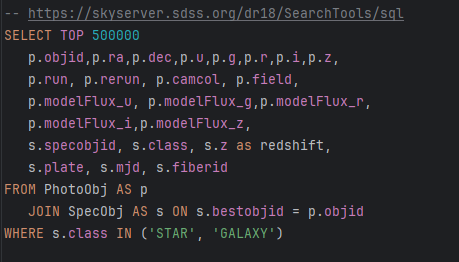
\includegraphics[width=100mm]{sql.png}
\caption{SQL upit korišćen za prikupljanje podataka sa SDSS sajta}
\label{fig:sql_query}
\end{figure}

Upitom je prikupljeno 500.000 redova. Spektar atributa dostupnih putem SDSS baze podataka mnogo je širi u poređenju sa SuperCOSMOS bazom, što omogućava detaljniju analizu i bolje treniranje modela. Na osnovu preporuka i primera sa njihovog sajta, izabrali smo određen broj ključnih atributa iz dostupnih tabela za dohvatanje podataka.

Pretprocesiranje podataka sa SDSS sajta pokazalo je znatno manji broj nedostajućih vrednosti i outlier-a u poređenju sa SuperCOSMOS Sky Survey skupom podataka. Nakon uklanjanja redova sa takvim anomalijama, preostalo je oko 492,000 redova koji su bili kvalitetni za dalju analizu. S obzirom na viši kvalitet podataka kao i veći broj slogova, dalji rad i analiza u ovom istraživanju fokusirani su na ovaj skup podataka.

\subsection{Učitavanje i čišćenje podataka}


\subsubsection{Učitavanje podataka}
Podaci su učitani korišćenjem biblioteke pandas, koja je moćan alat za manipulaciju i analizu podataka u Pythonu. Nakon učitavanja, proverili smo da li je skup podataka uspešno dovučen i uradili smo osnovne operacije za pregled podataka i njegove statistike. Takođe u ovom procesu su i isključene kolone koje nisu potrebne za dalju analizu i treniranje modela za klasifikaciju (više o izboru atributa u narednoj sekciji):

\begin{figure}[H]
\centering
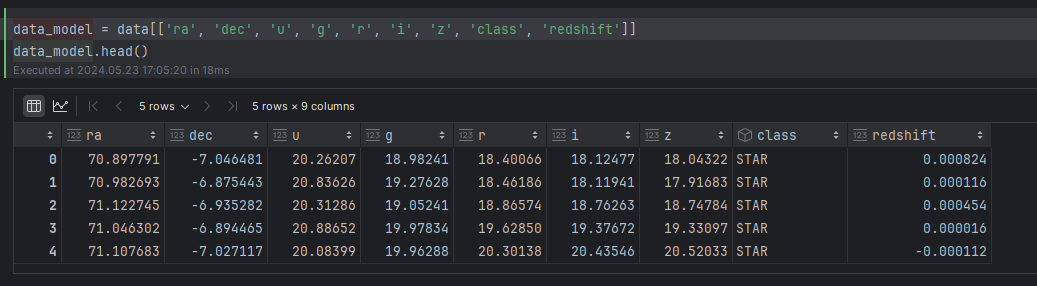
\includegraphics[width=150mm]{list_data.png}
\caption{Izlistavanje nekolicine redova učitanog skupa podataka}
\label{fig:sql_query}
\end{figure}

\subsubsection{Identifikacija i uklanjanje anomalija}
Proces čišćenja podataka je ključan korak u pripremi podataka za treniranje modela. Ovaj proces uključuje identifikaciju i razrešavanje anomalija, outlier-a i praznih vrednosti. S obzirom na količinu dostupnih podataka, a imajući i u vidu osetljivost u vrednostima atributa, strategija za razrešavanje u našem scenariju je bila jednostavno odstranjivanje redova sa takvim anomalijama\\\\
Prvo smo proverili da li skup podatak ima nedostajuće vrednosti u nekim kolonama:

\begin{figure}[H]
\centering
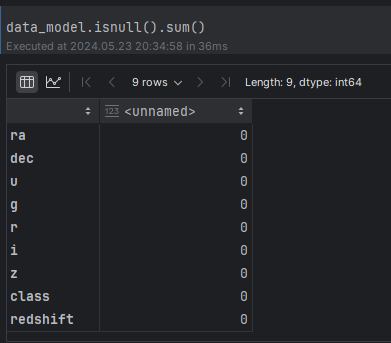
\includegraphics[width=80mm]{null_column_check.png}
\caption{Provera nedostajućih vrednosti u kolonama}
\label{fig:sql_query}
\end{figure}

Međutim, naš skup podataka nije imao takav slučaj pa smo obradu ovakvih redova preskočili.

\clearpage
Za uklanjanje outlier-a koristili smo algoritam Local Outlier Factor (LOF) za identifikaciju i uklanjanje outlier-a. LOF algoritam procenjuje udaljenost svakog podatka od njegovih suseda i identifikuje one podatke koji se značajno razlikuju od ostatka skupa.\\\\
Takođe, i bez algoritma jednostavnim pregledom osnovih statistika smo uvideli da neke kolone u sebi imaju određene anomalije:\\\\

\begin{figure}[H]
\centering
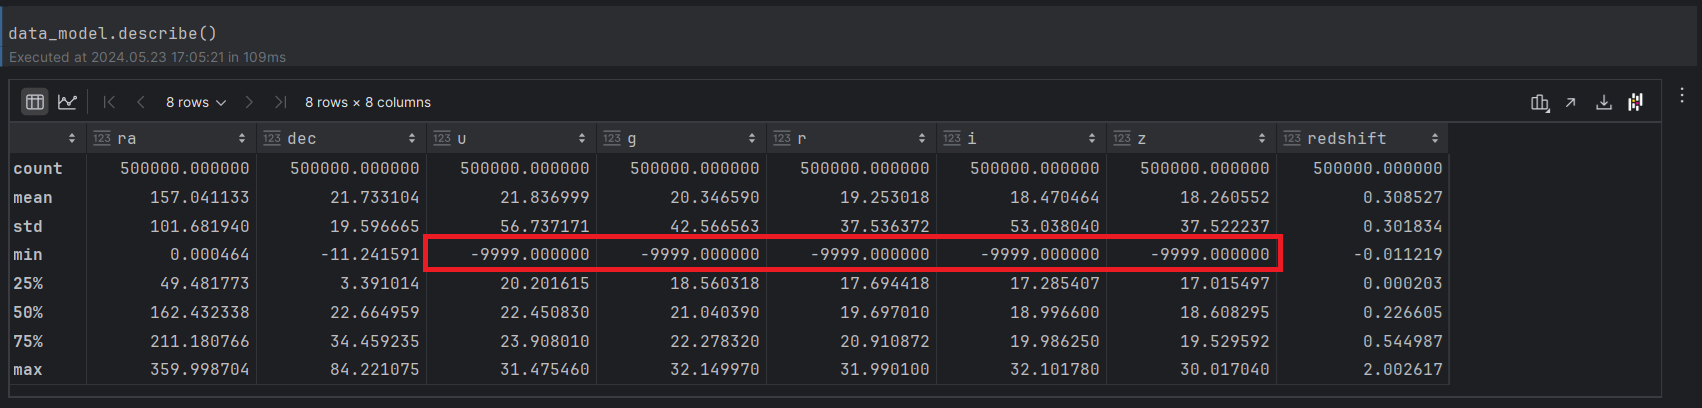
\includegraphics[width=160mm]{data_model_anomalies.png}
\caption{Prikaz osnovne statistike skupa podataka}
\label{fig:sql_query}
\end{figure}

Na slici se vidi da određeni broj kolona koji se odnosi na magniture ima vrednost od -9999.00 što je predstavljalo placeholder za redove koje imaju grešku ili su nepoznate.\\\\
Koraci u procesu čišćenja podataka uključivali su:
\begin{itemize}
    \item \textbf{Provera atributa}: Prvo je provereno da li skup podataka sadrži kategoričke atribute. Pošto su svi atributi numerički, svi atributi su uključeni u primeni algoritma za detekciju outlier-a.
    \item \textbf{Filtriranje outlier-a}: Na osnovu rezultata LOF algoritma, podaci identifikovani kao outlier-i su uklonjeni iz skupa podataka.
\end{itemize}
Korišćenjem ovog pristupa, uspeli smo da identifikujemo i uklonimo outlier-e iz skupa podataka, čime smo poboljšali kvalitet podataka za treniranje modela. Nakon čišćenja podataka, preostalo je 492,153 redova koji su bili kvalitetni za dalju analizu.

\begin{figure}[H]
\centering
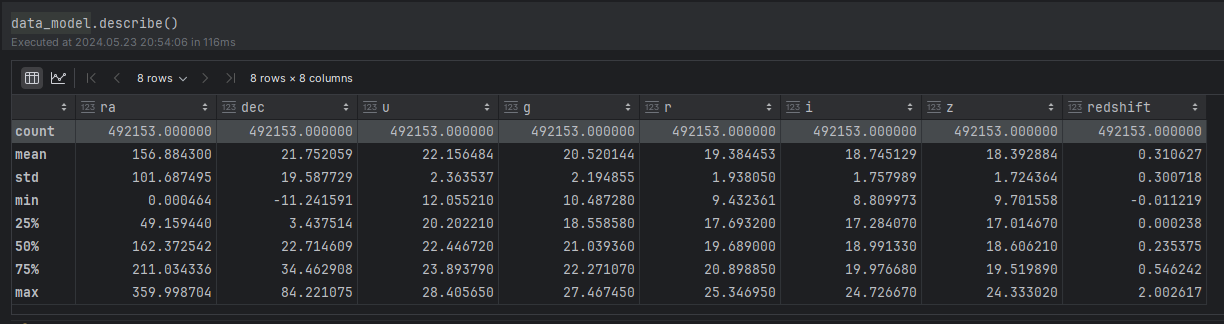
\includegraphics[width=160mm]{data_model_filtered.png}
\caption{Skup podataka nakon uklanjanja outlier-a}
\label{fig:sql_query}
\end{figure}

\clearpage
\subsection{Odabir atributa za treniranje modela}

Proces odabira atributa započeo je razumevanjem i analizom svakog atributa. Nakon toga, koristili smo različite grafičke prikaze kako bismo identifikovali koji atributi mogu biti najznačajniji za treniranje modela.\\\\

\subsubsection{Odstranivanje nepotrebnih atributa}

Za početak bez ikakve dodatne analize mogli smo da odstranimo neke atribute samo na osnovu njihovog značenja.

\noindent Atributi kao što su 'objid', 'run' i 'rerun' odnose se na administraciju podataka i nisu direktno bitni za izradu samog klasifikacionog modela.

\noindent Atributi 'camcol', 'field', 'plate' i 'fiberid' predstavljaju tehničke podatke koji se odnose na uslove pod kojima je snimljen nebeski objekat.

\noindent Atribut 'mjd' predstavlja modifikovani Julianov datum posmatranja i nije relevantan za određivanje da li je objekat zvezda ili galaksija.

\subsubsection{Izračunati atributi}

U razmatranje smo takođe uzeli u obzir i atribute koji nisu direktno dostupni u samom skupu podataka, ali se mogu izračunati i imaju određeno značenje u konkretnom domenu. Takvi atributi u našem slučaju su takozvani 'colour-indexes'.
\\\\Ovi atributi su izračunati na osnovu magnituda i predstavljaju razliku između sjaja u različitim delovima spektra. Oni pružaju dodatne informacije o karakteristikama nebeskih objekata.
        \begin{itemize}
            \item \textbf{color\_u\_g}: Razlika između magnituda u ultraljubičastom (u) i zelenom (g) delu spektra: $color\_u\_g = u - g$.
            \item \textbf{color\_g\_r}: Razlika između magnituda u zelenom (g) i crvenom (r) delu spektra: $color\_g\_r = g - r$.
            \item \textbf{color\_r\_i}: Razlika između magnituda u crvenom (r) i bliskom infracrvenom (i) delu spektra: $color\_r\_i = r - i$.
            \item \textbf{color\_i\_z}: Razlika između magnituda u bliskom infracrvenom (i) i dalekom infracrvenom (z) delu spektra: $color\_i\_z = i - z$.
        \end{itemize}

\subsubsection{RA \& DEC}

\begin{itemize}
    \item \textbf{RA (Right Ascension)}: Ovo je jedna od dve osnovne nebeske koordinate koje se koriste za određivanje položaja nebeskih objekata na nebeskoj sferi. RA se meri u satima, minutima i sekundama, i predstavlja ugaonu udaljenost objekta istočno od Prolećne tačke. RA je ekvivalent geografskoj dužini na Zemlji.
    
    \item \textbf{DEC (Declination)}: Druga osnovna nebeska koordinata koja se koristi za određivanje položaja objekata na nebeskoj sferi. DEC se meri u stepenima, minutima i sekundama, i predstavlja ugaonu udaljenost objekta severno ili južno od nebeskog ekvatora. DEC je ekvivalent geografskoj širini na Zemlji.
\end{itemize}

Sledeći grafikon prikazuje prostorni raspored zvezda i galaksija u ekvatorijalnim koordinatama. 

\begin{figure}[H]
\centering
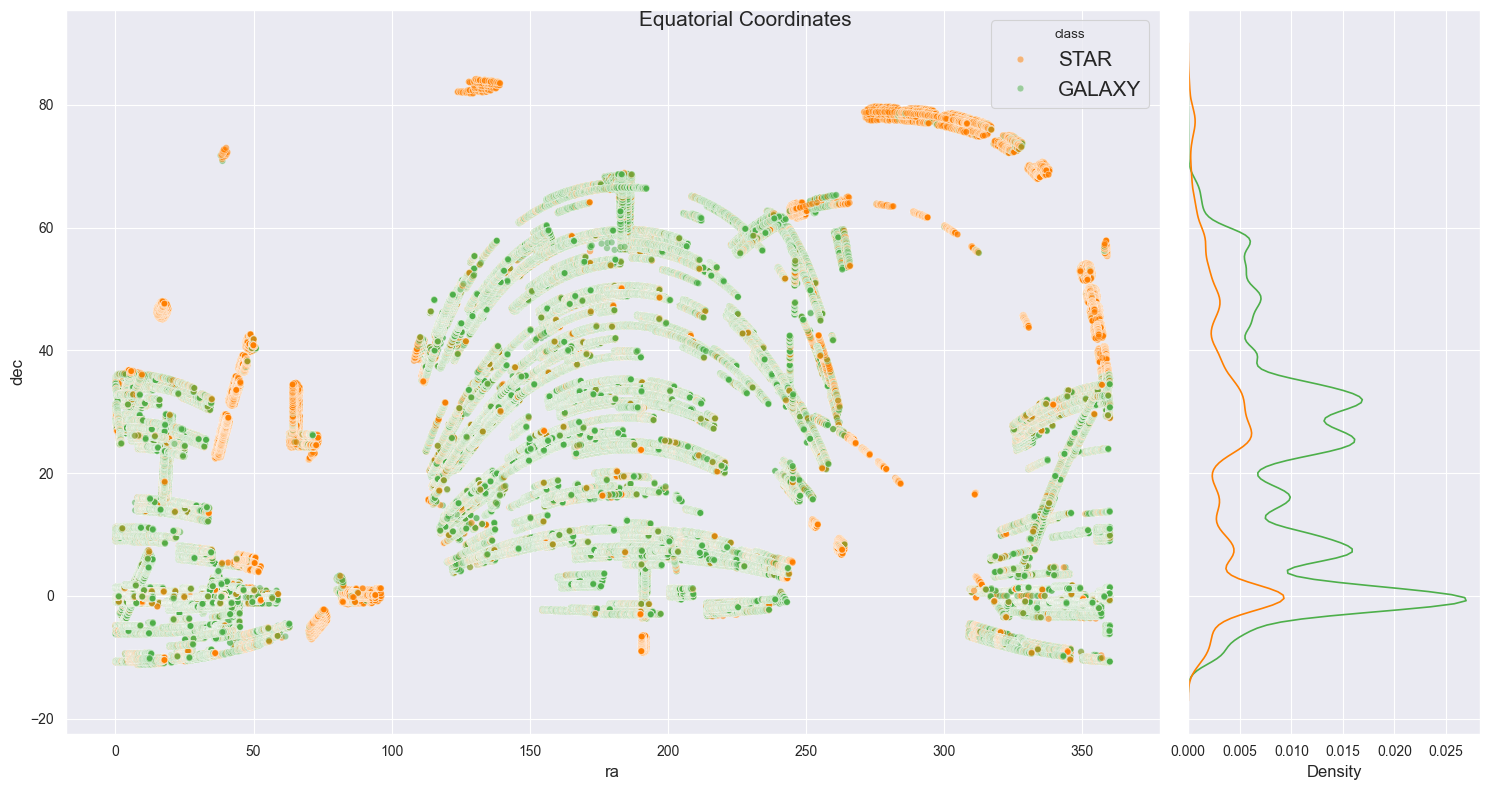
\includegraphics[width=150mm]{equatorial_coordinate_map.png}
\caption{Prostorni raspored zvezda i galaksija u ekvatorijalnim koordinatama}
\label{fig:equatorial_coordinates}
\end{figure}

Iz grafikona se može videti da:

\begin{itemize}
    \item Zvezde (narandžaste tačke) su raspoređene u određenim regijama, često u skupovima, što ukazuje na oblasti sa visokom koncentracijom zvezda.
    \item Galaksije (zelene tačke) su takođe raspoređene u skupovima, ali pokazuju drugačiji obrazac rasporeda u odnosu na zvezde.
    \item Gustinski graf na desnoj strani pokazuje da postoji razlika u raspodeli zvezda i galaksija duž deklinacije, što može pomoći u daljem istraživanju i klasifikaciji objekata.
\end{itemize}

\subsubsection{Magnituda}

Magnituda je mera sjaja nebeskog objekta viđenog sa Zemlje. Postoji pet filtera (u, g, r, i, z) koji mere sjaj u različitim delovima elektromagnetnog spektra:

\begin{itemize}
    \item \textbf{u (ultraljubičasti filter)}: Mera sjaja u ultraljubičastom delu spektra (354 nm).
    \item \textbf{g (zeleni filter)}: Mera sjaja u zelenom delu spektra (476 nm).
    \item \textbf{r (crveni filter)}: Mera sjaja u crvenom delu spektra (628 nm).
    \item \textbf{i (bliski infracrveni filter)}: Mera sjaja u bliskom infracrvenom delu spektra (769 nm).
    \item \textbf{z (daleki infracrveni filter)}: Mera sjaja u dalekom infracrvenom delu spektra (925 nm).
\end{itemize}
Značaj magnituda može se uočiti kroz prikaz odgovarajuće korelacione matrice za ove atribute.
\\\\Korelaciona matrica je vizualni prikaz koji pokazuje međusobnu povezanost različitih atributa korišćenih u skupu podataka.

\begin{figure}[H]
\centering
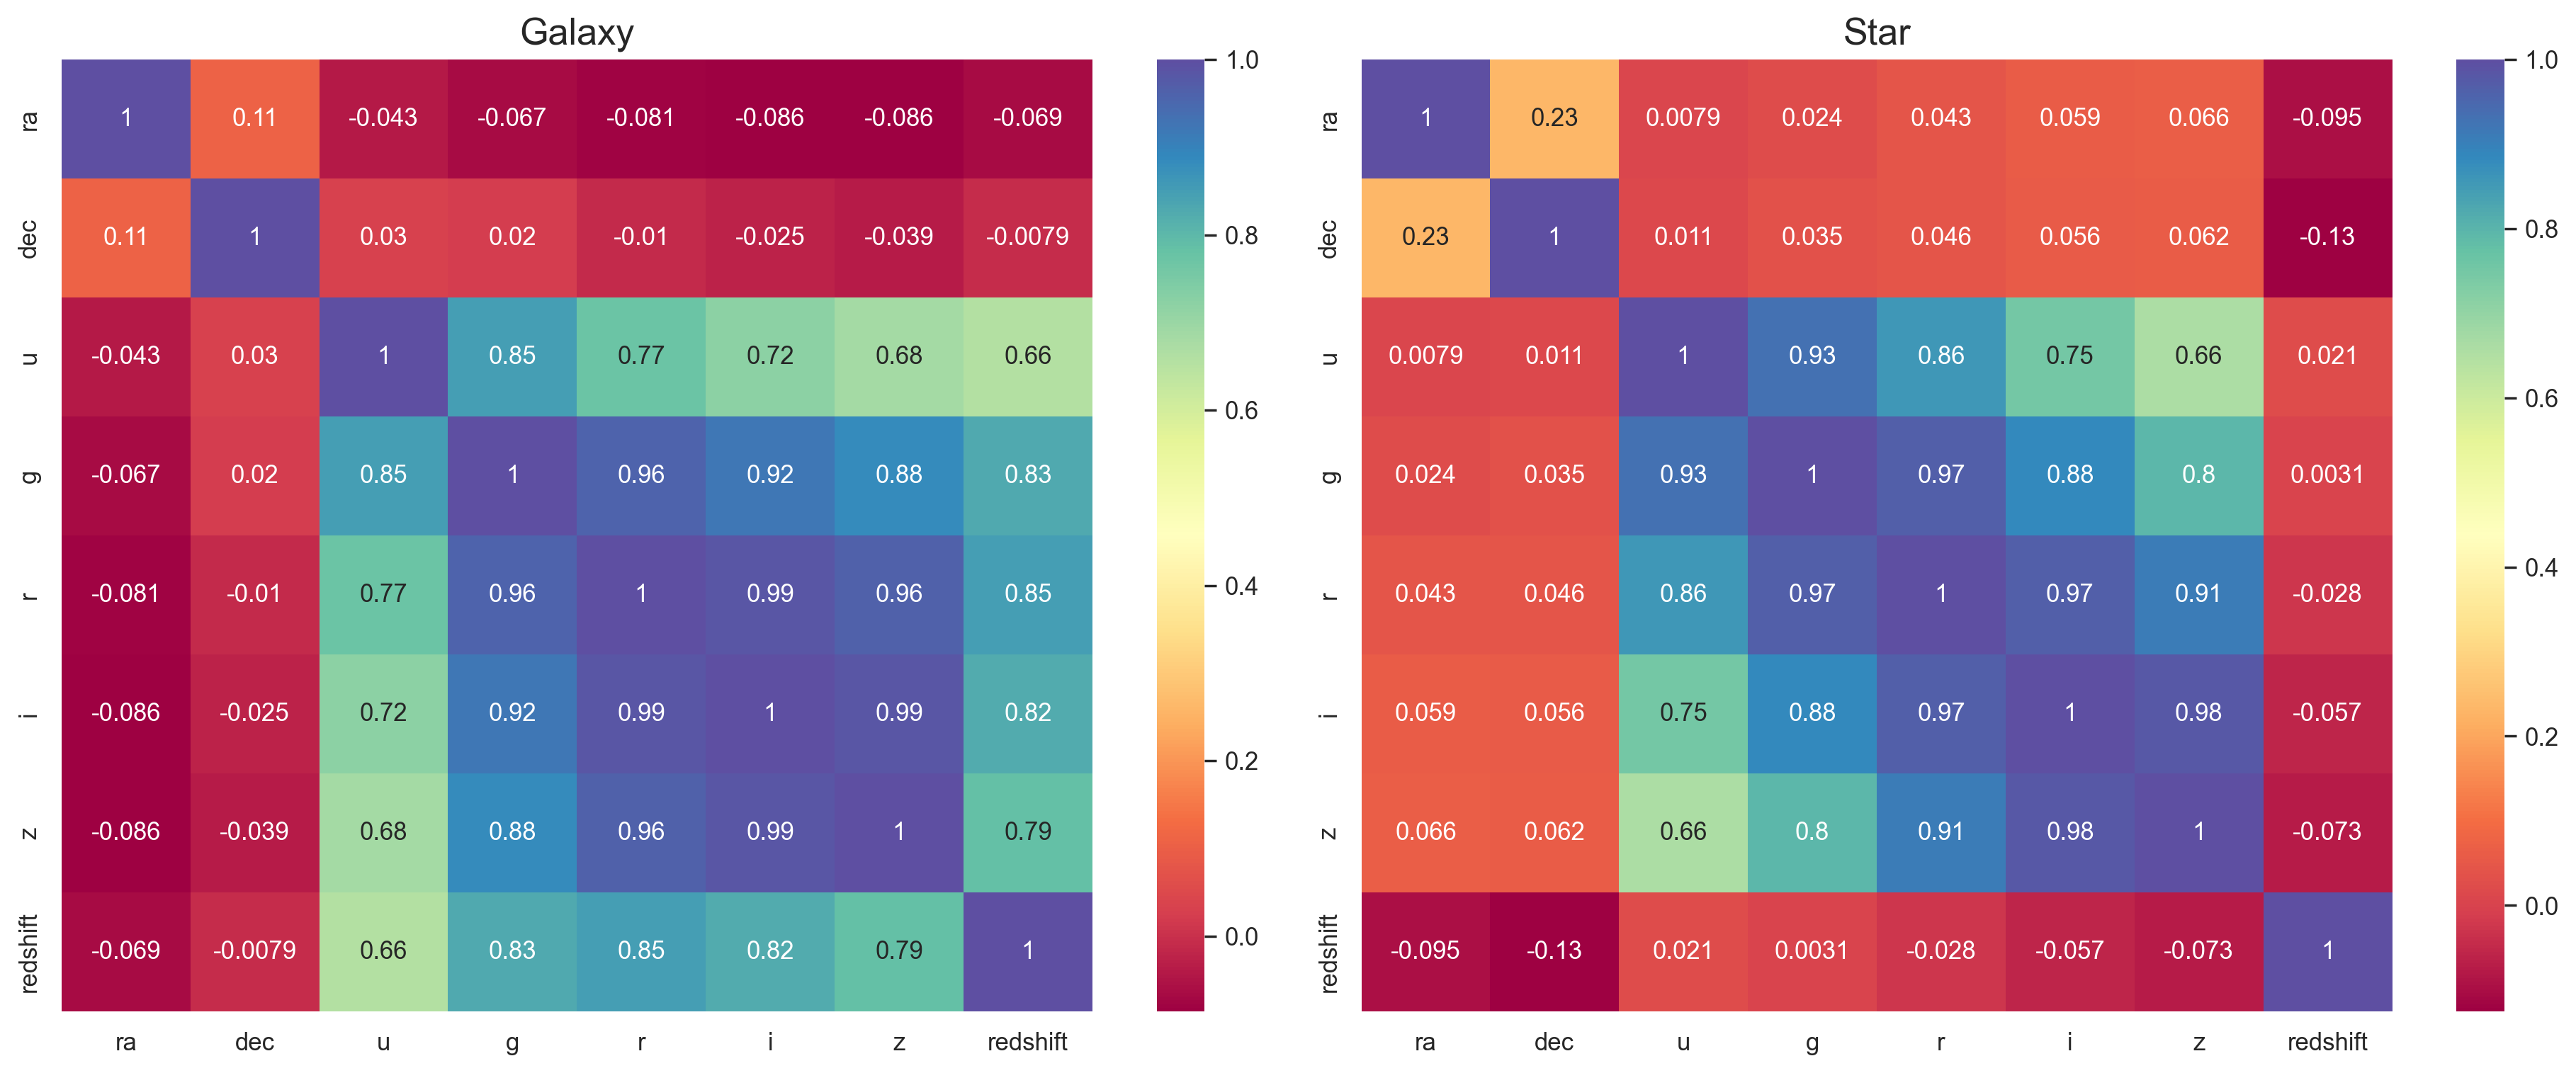
\includegraphics[width=120mm]{correlation_matrix.png}
\caption{Korelaciona matrica za atribute zvezda i galaksija}
\label{fig:correlation_matrix}
\end{figure}

Na grafikonu su prikazane korelacije između magnituda za zvezde (desno) i galaksije (levo).
\\Na prvi pogled možemo primetiti da su korelacione matrice veoma slične za obe klase (zvezde i galaksije). Možemo zaključiti da postoje visoke korelacije između različitih opsega. Ovo nije iznenađujuće; intuitivno, očekivali bismo da ako jedan opseg zabeleži svetlost nekog objekta, i ostali opsezi bi trebali zabeležiti svetlost. Međutim, interesantno je primetiti da je opseg 'u' manje povezan sa ostalim opsezima. Ovo je u skladu sa činjenicom da opsezi 'u', 'g', 'r', 'i', 'z' zabeležavaju svetlost na talasnim dužinama od 354, 476, 628, 769 i 925 nm, redom. Ovo može ukazivati da galaksije i zvezde sjaje jače na talasnim dužinama od 476 do 925 nm. Ipak, treba biti oprezan sa ovakvim interpretacijama.

\subsubsection{Redshift}
Crveni pomak je ključan fenomen u astronomiji jer omogućava određivanje udaljenosti i brzine udaljavanja nebeskih objekata, što je posebno važno za klasifikaciju između zvezda i galaksija. Razumevanje crvenog pomaka pomaže u identifikaciji galaksija koje se udaljavaju od nas zbog širenja svemira, dok zvezde, sa svojim karakterističnim relativnim brzinama unutar naše galaksije, pružaju dodatne informacije o njihovim kretanjima i položajima u odnosu na Sunčev sistem.


\begin{figure}[H]
\centering
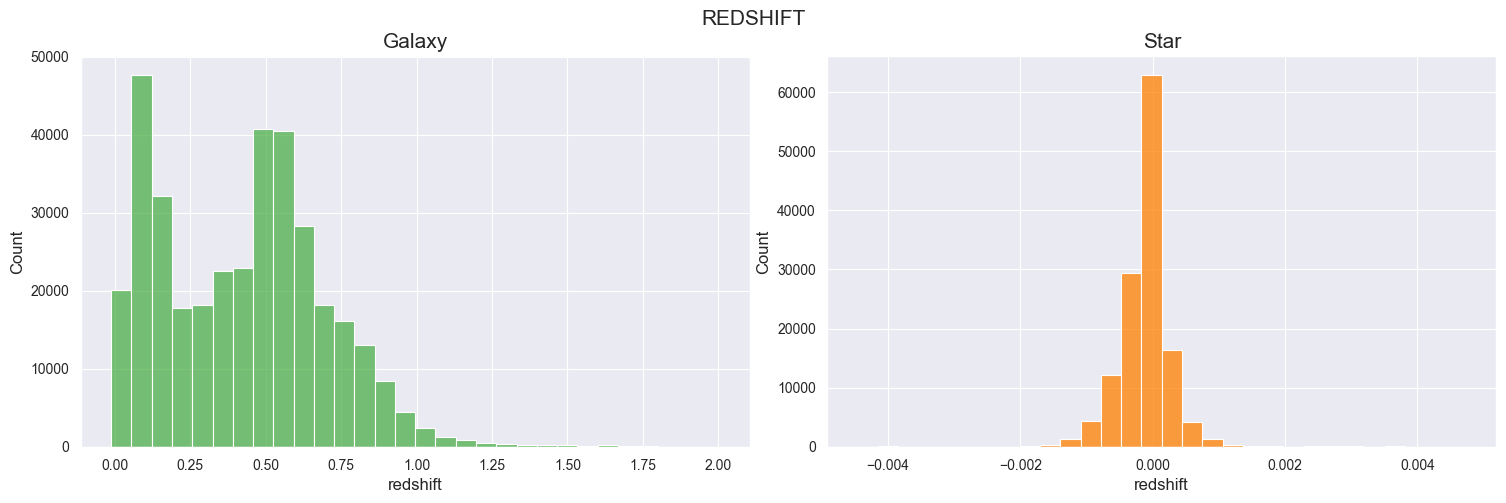
\includegraphics[width=150mm]{redshift_hist.png}
\caption{Histogram crvenog pomaka za zvezde i galaksije}
\label{fig:redshift_hist}
\end{figure}

Na slici \ref{fig:redshift_hist} prikazan je histogram crvenog pomaka za zvezde (desno) i galaksije (levo). Iz ovog histograma možemo zaključiti nekoliko važnih činjenica:

\begin{itemize}
    \item \textbf{Galaksije}: 
    \begin{itemize}
        \item Crveni pomak galaksija varira u širokom rasponu, od 0 do preko 2.0.
        \item Većina galaksija ima crveni pomak između 0.0 i 1.0, sa vrhom distribucije oko 0.5.
        \item Ovaj široki raspon crvenog pomaka potvrđuje da se galaksije udaljavaju različitim brzinama, što je u skladu sa Hablovim zakonom koji kaže da je brzina udaljavanja galaksija proporcionalna njihovoj udaljenosti od nas.
    \end{itemize}
    \item \textbf{Zvezde}: 
    \begin{itemize}
        \item Crveni pomak zvezda je veoma koncentrisan oko nule, sa većinom vrednosti između -0.004 i 0.004.
        \item Ova koncentracija oko nule ukazuje na to da se zvezde unutar naše galaksije kreću relativno malim brzinama u poređenju sa galaksijama, te se njihov crveni pomak uglavnom javlja zbog njihovih orbitalnih kretanja unutar naše galaksije.
    \end{itemize}
\end{itemize}
Crveni pomak može se koristiti kao procena udaljenosti objekta od Zemlje. Na osnovu histograma, većina posmatranih zvezda je bliža Zemlji nego galaksije. Galaksije su generalno dalje, što se može objasniti time da galaksije, zbog svoje veličine i fizičke strukture, emituju jače zračenje i mogu se posmatrati sa većih udaljenosti nego 'male' zvezde.
\\Kako možemo razlikovati klase objekata na osnovu kolone 'crveni pomak', ovaj atribut će verovatno biti od velike pomoći u klasifikaciji novih objekata.

\subsubsection{Class (klasa)}
Ovaj atribut označava klasifikaciju objekta kao zvezda ili galaksija. Ovo je ciljna promenljiva u klasifikacionom modelu.

\subsubsection{Zaključak}
Za treniranje klasifikacionih modela korišćeni su sledeći atributi: 'ra', 'dec', 'u', 'g', 'r', 'i', 'z', 'class', 'redshift', kao i izračunati atributi 'color\_u\_g', 'color\_g\_r', 'color\_r\_i', 'color\_i\_z'.

\clearpage


\subsection{Priprema podataka za treniranje modela}

Prvo što želimo da uradimo, želimo da proverimo koji je odnos klasa koje imamo u našem skupu podataka.

\begin{figure}[H]
\centering
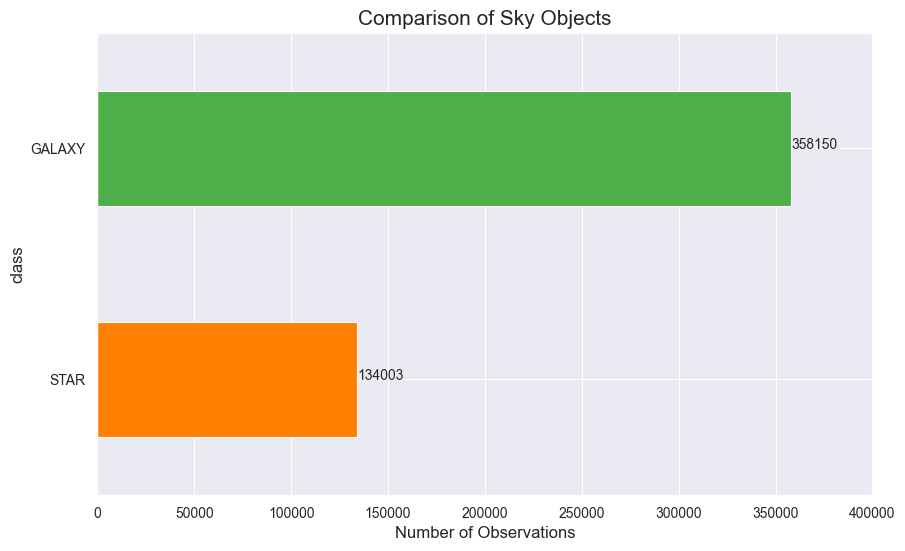
\includegraphics[width=120mm]{class_count_result.png}
\caption{Odnos klasa u skupu podataka}
\label{fig:sql_query}
\end{figure}

Vidimo da u skupu podataka imamo mnogo veći broj galaksija u odnosu na broj zvezda, svakako model ćemo trenirati nad svim dostupnim instancama.
\\\\Za uspešno treniranje i evaluaciju klasifikacionih modela, skup podataka je podeljen na dva dela: trening skup i test skup. Ovaj pristup omogućava pravilnu procenu performansi modela i njegovu generalizaciju na nove podatke.
\\\\Skup podataka je podeljen na sledeći način:
\begin{itemize}
    \item \textbf{Trening Skup (Training Set)}: Ovaj skup podataka se koristi za treniranje modela. Model uči obrasce i veze između atributa na osnovu ovog skupa.
    \item \textbf{Test Skup (Test Set)}: Ovaj skup se koristi za konačnu evaluaciju modela nakon što je treniran. Test skup pruža nezavisnu procenu performansi modela na novim, nepoznatim podacima.
\end{itemize}

Podaci su podeljeni tako da trening skup čini 75\% ukupnih podataka, i test skup preostalih 25\%. Ova podela je odabrana kako bi se osiguralo da ima dovoljno podataka za treniranje modela, ali i dovoljno za testiranje.\\\\
Takođe, prilikom podele podataka smo vodili pažnju da zadržimo originalni odnos zvezda i galaksija i u ovim podskupovima, kako ne bismo napravili trening i test skup koji su potencijalno još više disbalansirani.\\\\
Treba napomenuti da nismo unapred definisali i odredili validacioni skup, koji bismo koristili za korigovanje različitih hiperparametara kod različitih klasifikacionih algoritama. Umesto toga, koristili smo unakrsnu validaciju (cross-validation) kako bismo evaluirali performanse modela i optimizovali hiperparametre.

\subsubsection{Unakrsna validacija}
Unakrsna validacija je tehnika koja se koristi za procenu performansi modela i osiguravanje njegove generalizacije na nezavisnim skupovima podataka. U ovoj tehnici, prilikom treniranja modela, trening podaci se dele na $k$ podskupova (ili foldova). Model se trenira na $k-1$ podskupovima, a validira se na preostalom podskupu. Ovaj proces se ponavlja $k$ puta, tako da svaki podskup bude korišćen kao validacioni barem jednom. Na kraju, rezultati svih iteracija se agregiraju kako bi se dobila pouzdana procena performansi modela.\\\\
Korišćenjem unakrsne validacije, postigli smo nekoliko stvari:
\begin{itemize}
    \item \textbf{Optimizaciju hiperparametara}: Unakrsna validacija omogućava efikasno podešavanje hiperparametara modela bez potrebe za unapred definisanim validacionim skupom, što može povećati tačnost modela.
    \item \textbf{Bolju ocenu generalizacije}: Unakrsna validacija pomaže da se model generalizuje bolje na nezavisnim podacima jer koristi različite podskupove za treniranje i validaciju i samim tim možemo biti sigurniji da će se model ponašati slično i na testnim podacima kasnije.
\end{itemize}

\begin{figure}[H]
\centering
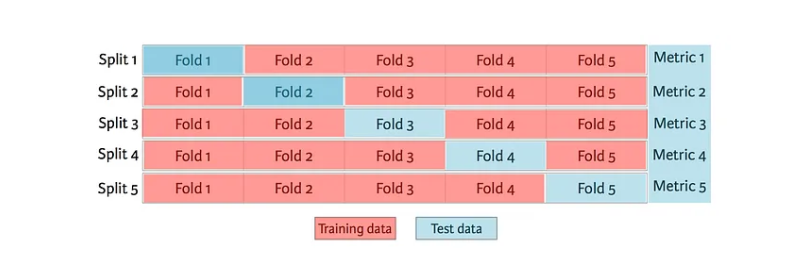
\includegraphics[width=120mm]{cross-validation.png}
\caption{Unakrsna validacija}
\label{fig:cross_validation}
\end{figure}

\subsubsection{Skaliranje Podataka}
Skaliranje podataka je ključan korak u pripremi podataka za treniranje modela. Podaci su standardizovani tako da imaju srednju vrednost 0 i standardnu devijaciju 1. Ovo je važno jer određeni algoritmi klasifikacije zahtevaju skalirane podatke kako bi se izbeglo da atributi sa većim opsegom vrednosti postanu automatski važniji od ostalih atributa. Skaliranje osigurava da svi atributi imaju jednaku težinu prilikom treniranja modela.\\\\
Skaliranje podataka je takođe značajno za mnoge optimizacione algoritme, kao što je gradijentni spust, jer doprinosi bržoj konvergenciji i stabilnijem učenju modela. Standardizacija podataka omogućava algoritmima da efikasnije pretražuju prostor rešenja, što rezultira boljim performansama i bržim treniranjem.
Još jedna bitna napomena jeste da podatke treba normalizovati nakon što ih podelimo na trening i test skupove kako bismo sprečili 'curenje podataka' koje bi modelu dalo dodatne informacije o test skupu ako bismo normalizovali sve podatke odjednom, a podelu podataka izvršili naknadno.

\section{Klasifikacioni Algoritmi}

\subsection{Metrike za Evaluaciju Modela}
Za evaluaciju performansi klasifikacionih modela korišćene su sledeće metrike: tačnost (accuracy), preciznost (precision), odziv (recall), F1-score i podrška (support). Ove metrike omogućavaju sveobuhvatnu procenu kvaliteta modela i njegove sposobnosti da tačno klasifikuje nebeske objekte kao zvezde ili galaksije.\\
Važno je napomenuti da je skup podataka neuravnotežen, sa većim brojem galaksija u odnosu na zvezde. U ovakvim situacijama, određene metrike, kao što su F1-score i odziv, postaju posebno važne za procenu performansi modela.

\begin{itemize}
    \item \textbf{Tačnost (Accuracy)}: Tačnost je mera koja pokazuje procenat tačno klasifikovanih instanci od ukupnog broja instanci. Visoka tačnost ukazuje na to da model dobro prepoznaje i zvezde i galaksije.
    \[
    \text{Tačnost} = \frac{\text{Broj tačno klasifikovanih instanci}}{\text{Ukupan broj instanci}}
    \]
    
    \item \textbf{Preciznost (Precision)}: Preciznost pokazuje koliko od svih instanci koje su modelom klasifikovane kao pozitivne (npr. zvezde) zaista pripada pozitivnoj klasi. Visoka preciznost znači da je mali broj lažno pozitivnih klasifikacija.
    \[
    \text{Preciznost} = \frac{\text{TP}}{\text{TP} + \text{FP}}
    \]
    gde su TP pravi pozitivni, a FP lažno pozitivni primerci.

    \item \textbf{Odziv (Recall)}: Odziv pokazuje koliko od svih stvarno pozitivnih instanci model tačno prepoznaje kao pozitivne. Visok odziv znači da je model sposoban da prepozna većinu pozitivnih instanci, što je posebno važno u neuravnoteženim datasetima gde je potrebno identifikovati što više pozitivnih instanci.
    \[
    \text{Odziv} = \frac{\text{TP}}{\text{TP} + \text{FN}}
    \]
    gde su TP pravi pozitivni, a FN lažno negativni primerci.

    \item \textbf{F1-score}: F1-score je harmonijska sredina preciznosti i odziva i koristi se kao jedinstvena mera performansi modela, naročito kada postoji neuravnoteženost klasa. F1-score uzima u obzir i preciznost i odziv, pružajući balansiranu meru performansi modela.
    \[
    \text{F1-score} = 2 \cdot \frac{\text{Preciznost} \cdot \text{Odziv}}{\text{Preciznost} + \text{Odziv}}
    \]

    \item \textbf{Podrška (Support)}: Podrška označava broj instanci u svakoj klasi u skupu podataka. Koristi se za procenu uravnoteženosti klasa i može uticati na izbor metrika za evaluaciju modela.
\end{itemize}

Uz ove metrike, koristili smo i matricu konfuzije za dodatnu evaluaciju modela. Matrica konfuzije je tabela koja prikazuje stvarne klase naspram predviđenih klasa, omogućavajući identifikaciju tačno i pogrešno klasifikovanih instanci. Redovi matrice predstavljaju stvarne klase, dok kolone predstavljaju predviđene klase. Matrica konfuzije pomaže u vizualizaciji performansi modela i identifikaciji specifičnih vrsta grešaka, kao što su lažno pozitivni i lažno negativni primerci.\\\\


\subsection{Stabla odlučivanja}
Decision tree (stablo odluke) je jedan od najjednostavnijih i najintuitivnijih algoritama za klasifikaciju. Radi tako što deli podatke na osnovu vrednosti atributa i pravi hijerarhijsku strukturu odluka, gde svaka grana predstavlja ishod odluke, a svaki čvor predstavlja atribut po kojem se podaci dele.


\subsubsection{Trening}

Za treniranje Decision Tree modela korišćen je skup podataka koji je prethodno podeljen na trening i test skup. Za treniranje modela nije bilo potrebno koristiti skalirane podatke, jer Decision Tree algoritmi ne zavise od udaljenosti između tačaka.

Decision Tree algoritmi imaju različite hiperparametre koji mogu uticati na kvalitet modela. Neki od tih hiperparametara uključuju maksimalnu dubinu stabla, minimalan broj uzoraka potrebnih za podelu čvora, minimalan broj uzoraka u listu i broj karakteristika koje se koriste za traženje najbolje podele.

Da bismo pronašli najbolju kombinaciju hiperparametara, koristili smo GridSearchCV funkciju iz paketa scikit-learn. Ova funkcija automatski pretražuje različite kombinacije hiperparametara i procenjuje performanse modela za svaku od njih. Na ovaj način možemo identifikovati konfiguraciju hiperparametara koja daje najbolje rezultate za dati skup podataka.\\
Jedan od parametara koji se prosleđuje GridSearchCV funkciji je metrika koja će se koristiti za procenu kvaliteta modela tokom pretrage. U našem slučaju, koristili smo tačnost (accuracy).\\
Važno je napomenuti da GridSearchCV koristi unakrsnu validaciju (cross-validation) kako bi procenio performanse modela u svakoj iteraciji pretrage. Za naše modele smo koristili 10-fold unakrsnu validaciju, što znači da je skup podataka podeljen na 10 delova, pri čemu se model trenira 10 puta, svaki put koristeći drugačiji deo kao test skup, a preostalih 9 delova kao trening skup.\\
Mana ovog pristupa je što može biti vremenski zahtevan, jer se broj treniranja modela (fitova) računa kao broj mogućih kombinacija hiperparametara pomnožen sa brojem foldova.\\
Nakon što smo identifikovali najbolji skup hiperparametara, iskoristili smo ih da ponovo istreniramo model, ali ovog puta koristeći ceo trening skup podataka.

\begin{figure}[H]
\centering
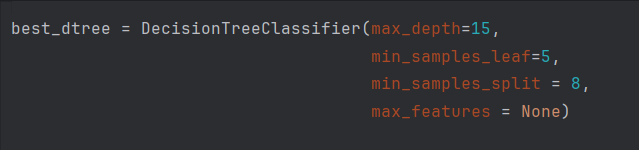
\includegraphics[width=150mm]{best_dtree.png}
\caption{Najbolji parametri za model stabla odlučivanja}
\label{fig:best_dtree}
\end{figure}

\subsubsection{Rezultati}

Nakon optimizacije hiperparametara, model je evaluiran na test skupu podataka. Rezultati pokazuju visoku tačnost i odlične metrike za klasifikaciju.

\begin{figure}[H]
\centering
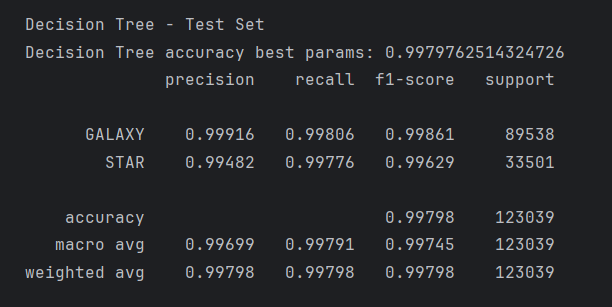
\includegraphics[width=90mm]{decision_tree_classification_report.png}
\caption{Rezultati klasifikacije stabla odlučivanja na test skupu}
\label{fig:decision_tree_classification_report}
\end{figure}

Rezultati pokazuju da je model stabla odlučivanja vrlo efikasan u klasifikaciji nebeskih objekata, sa visokim vrednostima preciznosti, odziva i F1-score-a za obe klase.

\begin{figure}[H]
\centering
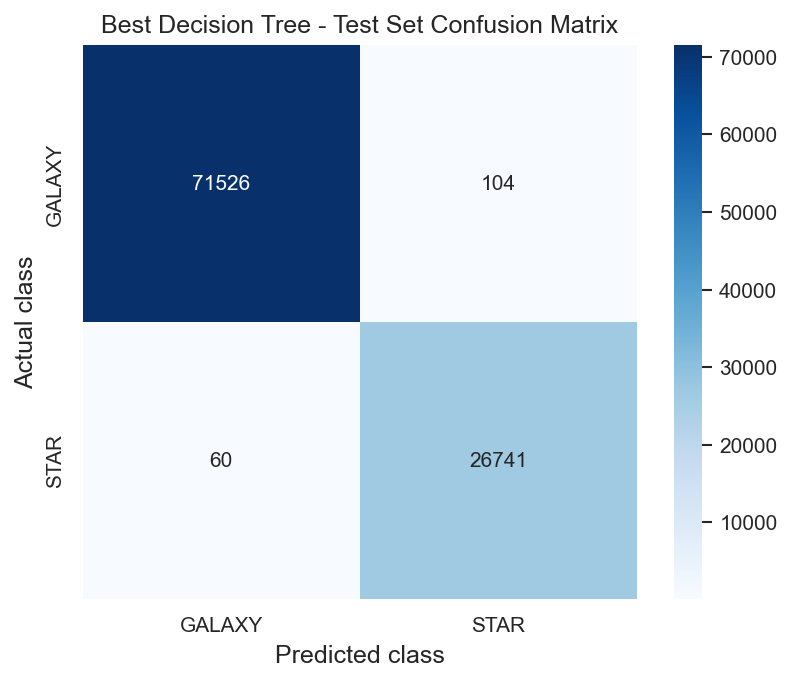
\includegraphics[width=90mm]{decision_tree_cm.png}
\caption{Matrica konfuzije za model stabla odlučivanja na test skupu}
\label{fig:decision_tree_cm}
\end{figure}

Matrica konfuzije pruža dodatni uvid u rezultate evaluacije modela, prikazujući tačne i netačne klasifikacije za svaku klasu.
\\\\Ovi rezultati potvrđuju da algoritam stabla odlučivanja može biti izuzetno efikasan za klasifikaciju nebeskih objekata, pružajući visok nivo tačnosti i pouzdanosti.

\subsection{Logistička regresija}
Logistička regresija (logistic regression) je popularan algoritam za binarnu klasifikaciju koji modelira verovatnoću da primerak pripada određenoj klasi. Algoritam koristi logističku funkciju za predikciju verovatnosti, a zatim klasifikuje primerke na osnovu praga verovatnoće (obično 0.5).

\subsubsection{Treniranje i evaluacija}
Za treniranje modela korišćen je skup podataka koji je prethodno podeljen na trening i test skup. Podaci su skalirani kako bi se obezbedila bolja konvergencija i kvalitet modela.

Kako bismo dodatno poboljšali kvalitet modela i smanjili varijansu, korišćena je unakrsna validacija.

\subsubsection{Rezultati Unakrsne Validacije}
Prosečna tačnost modela procenjena unakrsnom validacijom je pokazala visok nivo tačnosti, sa malim standardnim odstupanjem, što ukazuje na konzistentne performanse modela.

\begin{verbatim}
Mean Accuracy: 0.99019 (0.001)
\end{verbatim}

\subsubsection{Rezultati}

\begin{figure}[H]
\centering
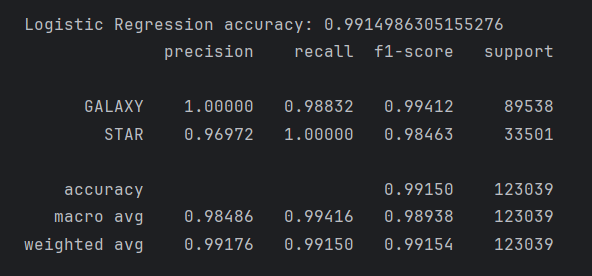
\includegraphics[width=90mm]{logistic_regression_classification_report.png}
\caption{Rezultati klasifikacije modela na test skupu}
\label{fig:logistic_regression_classification_report}
\end{figure}

\begin{figure}[H]
\centering
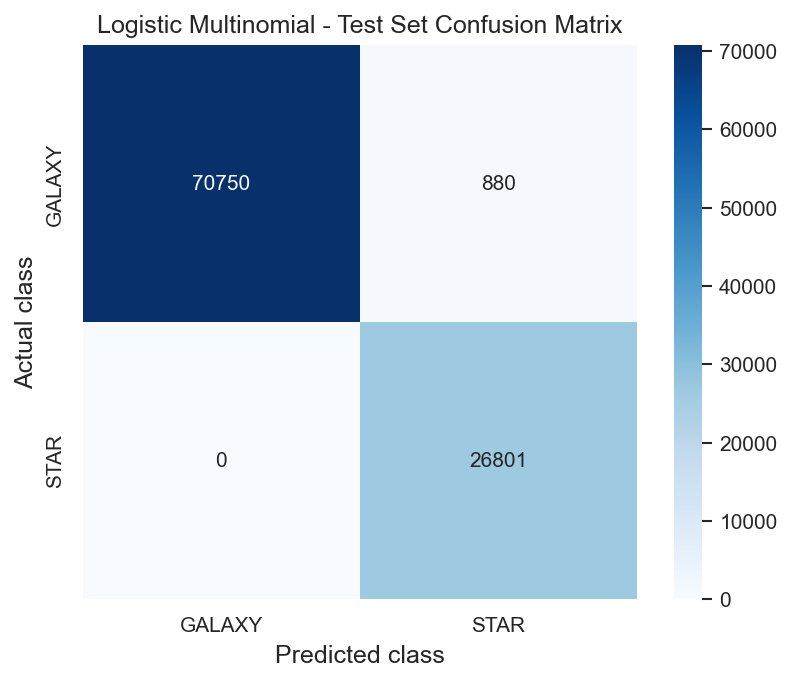
\includegraphics[width=90mm]{logistic_regression_cm.png}
\caption{Matrica konfuzije za Logistic Regression model na test skupu}
\label{fig:logistic_regression_cm}
\end{figure}

Iako ovaj model postiže dobre sveobuhvatne metrike, kao što su visoka tačnost, preciznost i odziv, primećeno je da ima tendenciju grešaka u klasifikaciji galaksija. Konkretno, model često pogrešno klasifikuje galaksije kao zvezde, što je prikazano u matrici konfuzije na slici \ref{fig:logistic_regression_cm}.\\\\
Ova greška može biti značajna u određenim aplikacijama, čime stabla odlčivanja postaju bolji izbor za ovaj zadatak zbog veće preciznosti u razlikovanju klasa.

\subsection{K-najbližih suseda}

K-najbližih suseda (KNN) je jednostavan, ali moćan algoritam mašinskog učenja koji se koristi za zadatke klasifikacije i regresije. U ovom radu koristićemo ga za klasifikaciju. KNN ne gradi globalni model, već koristi primere iz trening skupa za pravljenje predikcija za test instance. Takvi algoritmi zahtevaju meru blizine kako bi odredili sličnost ili udaljenost između instanci i funkciju klasifikacije koja vraća predviđenu klasu test instance na osnovu njene blizine drugim instancama. Neke od mera udaljenosti koje se koriste za pronalaženje najbližeg suseda su: Euklidsko rastojanje, rastojanje Minkovskog, Hamingovo rastojanje i Menhetn rastojanje.

\subsubsection{Normalizacija podataka}
Kod KNN algoritma neophodno je da su podaci normalizovani, zato što algoritam koristi meru za udaljenost između tačaka.

\subsubsection{Prilagođavanje i evaluacija modela}
Za prilagođavanje KNN modela, koristili smo grid pretragu u kombinaciji sa unakrsnom validacijom kako bismo optimizovali vrednosti hiperparametara. Izbor vrednosti 'k' igra ključnu ulogu u performansama KNN modela. Klasifikator sa malim brojem suseda može dovesti do preprilagođavanja, dok model sa mnogo suseda može dovesti do nedovoljno prilagođenog modela.
\\\\Ukoliko vizualizujemo sad performanse modela za različite vrednosti k na trening podacima, najbolje performanse su koristeći oko 6 suseda. Što je broj suseda veći to model postaje jednostavniji i tačnost na trening skupu opada. Međutim, ako pogledamo y-osu, razlika između tačnosti nije velika i bilo koja vrednost 'k' bi dobro obavila posao na našem problemu jer je najgora performansa oko 0.976.

\begin{figure}[H]
\centering
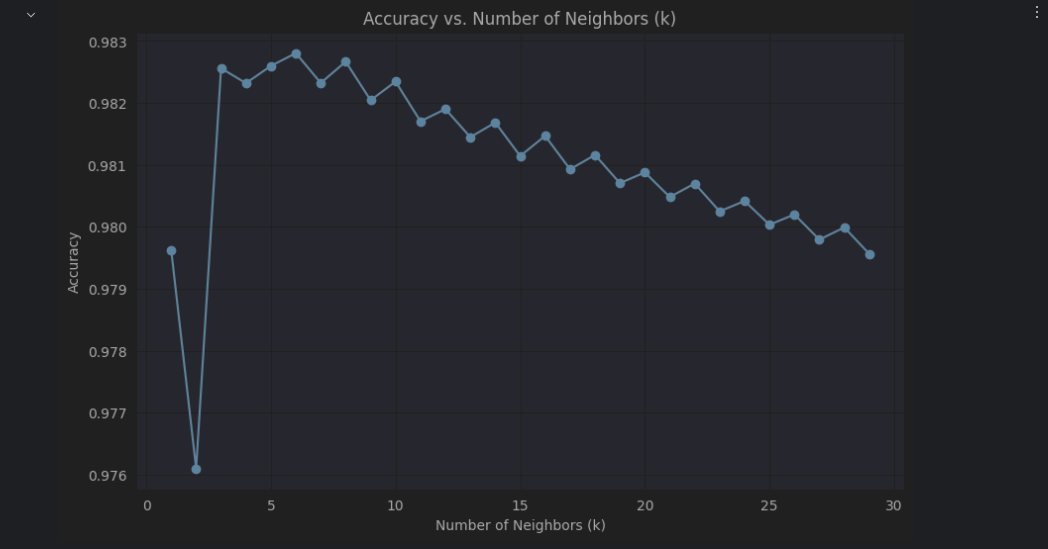
\includegraphics[width=90mm]{knn_accuracy_vs_knn.png}
\caption{Odnos performansi modela i broja suseda}
\label{fig:knn_accuracy_vs_knn}
\end{figure}

Slično kao i kod prethodnih modela, za traženje najboljeg skupa hiperparametara koristili smo grid pretragu u kombinaciji sa unakrsnom validacijom.
\\\\Kako bismo poboljšali model optimizujemo tri glavna hiperparametra koja utiču na prilagođavanje modela: n\textunderscore neighbours, weights i metric. Svi ostali hiperparametri ostaju na svojim podrazumevanim vrednostima.
\begin{verbatim}
    param_grid = {
        "n_neighbors": np.arange(1,12),
        "weights": ['uniform', 'distance'],
        "metric": ["euclidean","manhattan"],
        "n_jobs": [4]
    }
\end{verbatim}
\begin{itemize}
    \item \textbf{n\textunderscore neighbors}: Ovo predstavlja broj najbližih suseda koje k-NN algoritam treba da uzme u obzir.
    \item \textbf{weights}: Ovo određuje način na koji se računa doprinos svakog suseda. Postoje dve opcije:
    \begin{itemize}
        \item \textbf{uniform}: Svi susedi imaju isti doprinos bez obzira na udaljenost
        \item \textbf{distance}: Susedi bliži tački imaju veći doprinos nego udaljeni susedi.
    \end{itemize}
    \item \textbf{metric}: Ovo određuje način na koji se meri udaljenost između tačaka. Postoje dve opcije:
    \begin{itemize}
        \item \textbf{euclidean}
        \item \textbf{manhattan}
    \end{itemize}
    \item n\textunderscore jobs: Ovo određuje broj paralelnih zadataka koje treba pokrenuti prilikom obrade. Vrednost 4 znači da će se koristiti četiri procesorska jezgra za paralelnu obradu.
\end{itemize}
Rezultati su pokazali da je najbolja kombinacija parametara
\begin{verbatim}
    Best params: {'metric': 'manhattan',
              'n_neighbors': 6,
              'weights': 'uniform'}
    Best score:  0.9835416993884458
\end{verbatim}

Nakon što smo odradili optimizaciju modela vreme je da pokrenemo najbolje dobijen model na test podacima i da vidimo kolika će biti uspešnost modela.

\subsubsection{Rezultati}

\begin{figure}[H]
\centering
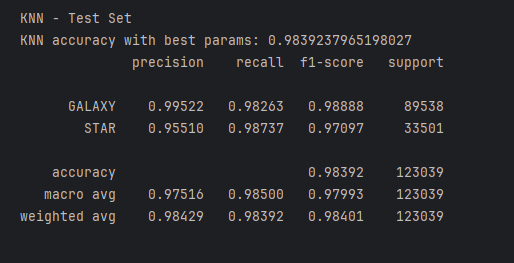
\includegraphics[width=90mm]{knn_classification_result.png}
\caption{Rezultati KNN modela na test skupu}
\label{fig:knn_classification_result}
\end{figure}

\begin{figure}[H]
\centering
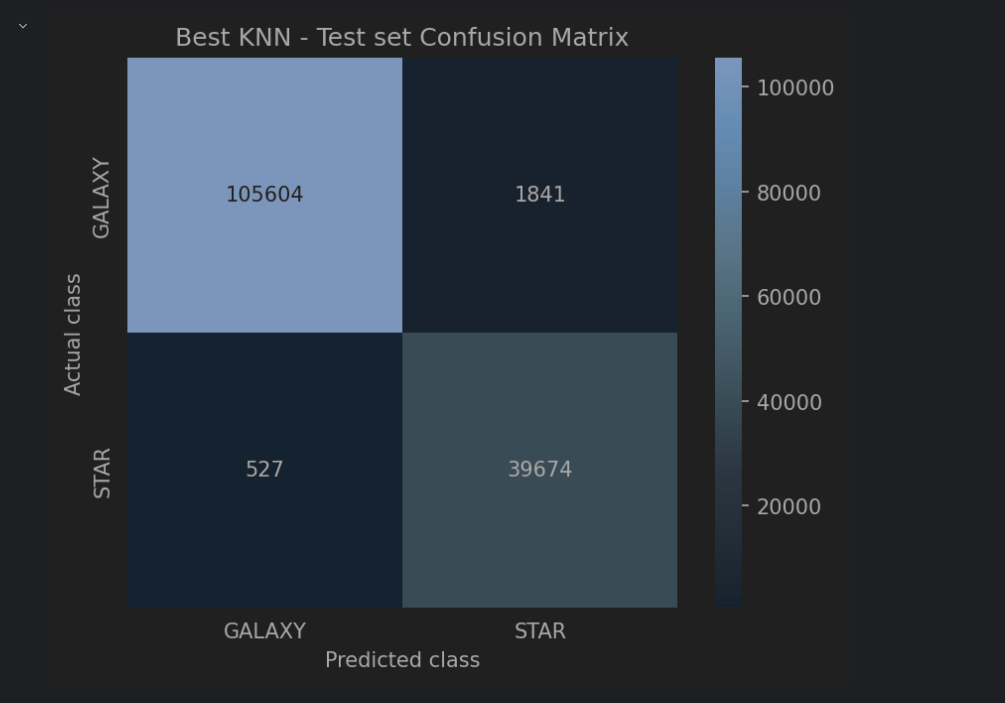
\includegraphics[width=90mm]{knn_cm.png}
\caption{Matrica konfuzije za KNN model na test skupu}
\label{fig:knn_cm}
\end{figure}

Vidimo da ovaj model postiže lošije rezultate u odnosu na prvobitna dva algoritma.

\subsection{Slučajna šuma}
Metod slučajnih šuma se zasniva na prostoj agregaciji stabala odlučivanja. Ansambl (skupovi većeg broja modela koji zajednički donose odluke) se sastoji od m stabala treniranih na različitim podskupovima skupa za obučavanje. Jedno stablo se obučava tako što se izabere podskup skupa za obučavanje odredene veličine, pri čemu je moguće koristiti i samo podskup ukupnog skupa atributa. Stabla se obučavaju na različitim podskupovima kako bi njihove greške bile što slabije korelisane, što ostavlja prostor za popravku agregacijom.
\\\\Slučajne šume su jedan od najprimenjenijih algoritama mašinskog učenja.
Njihovo obučavanje je relativno efikasno, a preciznost predvidjanja obično među
najboljim za vektorski predstavljene podatke. Njegova jednostavnost korišćenja i fleksibilnost doprineli su njegovoj popularnosti, jer može da rešava i klasifikacione i regresione probleme. Neki od nedostataka upotrebe algoritma slučajne šume su: zahteva više resursa za obradu, troši više vremena u poređenju sa algoritmom stabla odluke, manje je intuitivan kada imamo veliki broj stabala odluke, izuzetno je složen i zahteva više računske snage..

\subsubsection{Treniranje modela}
Kao i kod prethodnih algoritama, koristili smo prethodno podeljene skupove za trening i test. Korišćenje slučajne šume obično ne zahteva skaliranje podataka. Algoritmi za slučajne šume, kao i drugi algoritmi bazirani na stablima odluke, nisu osetljivi na skalu ili distribuciju podataka.

\subsubsection{Optimizacija modela}
Hiperparametri se koriste u slučajnim šumama da bi se poboljšale performanse i prediktivna moć modela ili da bi model bio brži.
Hiperparametri na koje smo se odlučili da se fokusiramo su:
\begin{itemize}
    \item \textbf{n\textunderscore estimators} - broj stabala u šumi
    \item \textbf{max\textunderscore features} - maksimalan broj atributa korišćenih pri podeli čvora, obično manji od broja atributa u skupu podataka
    \item \textbf{max\textunderscore depth} - maksimalan broj nivoa u svakom stablu odluke
    \item \textbf{min\textunderscore samples\textunderscore split} - minimalan broj podataka u čvoru pre nego što se čvor podeli
    \item \textbf{min\textunderscore samples\textunderscore leaf} - minimalan broj podataka dozvoljen u listu
    \item \textbf{criterion} - funkcija za merenje kvaliteta podele
\end{itemize}

Postoji nekoliko tehnika optimizacije hiperparametara za algoritam slučajne šume, kao što su grid pretraga, Bajesova optimizacija i nasumična pretraga. Za razliku od grid pretrage, za podešavanje hiperparametara zasnovano na nasumičnoj pretrazi se ne koriste sve moguće kombinacije hiperparametara. Grid pretraga iscrpno pretražuje svaku kombinaciju unapred definisanih vrednosti hiperparametara, što značajno povećava vreme obrade. Međutim, nasumična pretraga uzima uzorak konstantne veličine konfiguracija hiperparametara određenih raspodelom njihovih vrednosti. Korišćenje nasumične pretrage omogućava pronalaženje raznovrsnije regije hiperparametara. Iako ne garantuje pronalaženje hiperparametara koji čine najbolju kombinaciju, dovoljno je dobra da brzo postigne vrlo dobru kombinaciju, što je posebno važno kada se radi sa skupovima podataka u astronomiji, gde obično postoji veliki broj opservacija, što generiše značajno vreme obrade.

Izvršili smo nasumičnu pretragu hiperparametara koristeći unakrsnu validaciju (cv=10), kroz 100 različitih kombinacija (n\textunderscore iter=100), i sa svim dostupnim jezgrima istovremeno (n\textunderscore jobs=-1). Nasumična pretraga nasumično bira kombinaciju hiperparametara umesto iteriranja kroz svaku moguću kombinaciju. Veći n\textunderscore iter i cv rezultiraju većim brojem kombinacija i manjom mogućnošću prekomernog prilagođavanja. U svakoj iteraciji, algoritam će odabrati različitu kombinaciju hiperparametara.\\\\
Najbolji hiperparametara koji su dobijeni nasumičnom pretragom
\begin{verbatim}
    {
     'n_estimators': 100,
     'min_samples_split': 5,
     'min_samples_leaf': 2,
     'max_features': None,
     'max_depth': 15,
     'criterion': 'entropy'
    }
\end{verbatim}

\subsubsection{Rezultati}

\begin{figure}[H]
\centering
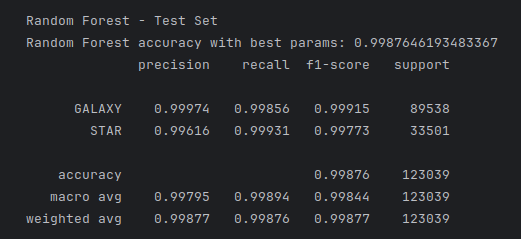
\includegraphics[width=90mm]{random_forest.png}
\caption{Rezultati Slucajne sume na test skupu}
\label{fig:random_forest}
\end{figure}

\begin{figure}[H]
\centering
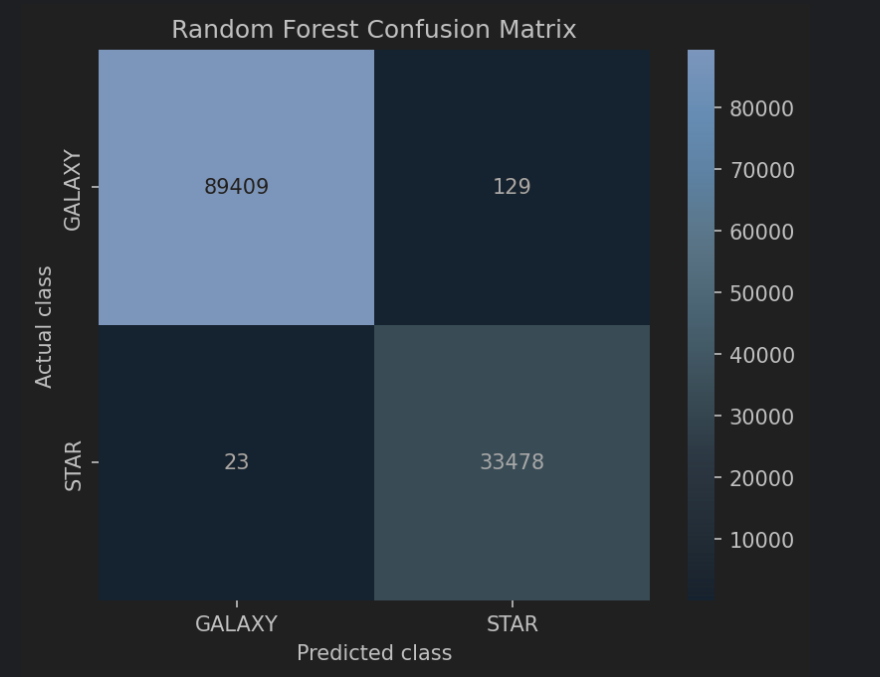
\includegraphics[width=90mm]{random_forest_cm.png}
\caption{Matrica konfuzije za Slucajnu sumu na test skupu}
\label{fig:random_forest_cm}
\end{figure}

Još jedna od dobrih karakteristika slučajne šume jeste što možemo da odredimo važnost svakog pojedinačnog atributa.

\begin{figure}[H]
    \centering
    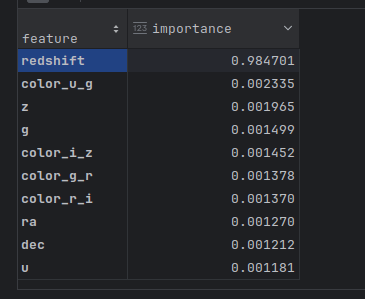
\includegraphics[width=80mm]{feature_importance.png}
    \caption{Važnost atributa}
    \label{fig:feature_importance}
\end{figure}

Možemo primetiti da je redshift najvažniji atribut od svih kao što smo i pretpostavili na početku na osnovu histograma.
\\\\Takođe vidimo da do sada, ovaj klasifikacioni algoritam daje najbolje rezultate.

\subsection{Naive Bayes (Gaus)}
Gaussian Naive Bayes (GNB) je algoritam za klasifikaciju zasnovan na Bayesovoj teoremi sa pretpostavkom da su karakteristike podjednako i nezavisno normalno distribuirane. Ovaj algoritam je jednostavan za implementaciju i efikasan, posebno za visoko-dimenzionalne podatke.

\subsubsection{Treniranje i Evaluacija}
Treniranje i evaluacija Gaussian Naive Bayes modela izvedeni su korišćenjem pretrage za optimizaciju hiperparametara. Hiperparametar \textit{var\_smoothing}, koji dodaje varijansu na procene verovatnoće kako bi se stabilizovale procene, optimizovan je korišćenjem unakrsne validacije (cross-validation) sa deset preklopnih skupova (foldova).

\subsubsection{Rezultati}
Nakon optimizacije hiperparametara, Gaussian Naive Bayes model je evaluiran na test skupu podataka. Rezultati su prikazani u sledećim slikama.

\begin{figure}[H]
\centering
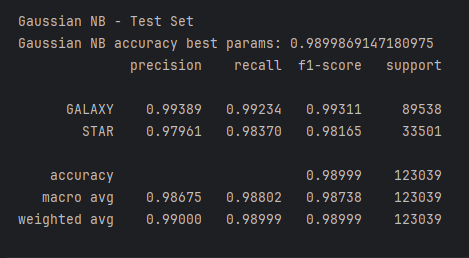
\includegraphics[width=90mm]{gaussian_nb_classification_report.png}
\caption{Rezultati klasifikacije Gaussian Naive Bayes modela na test skupu}
\label{fig:gaussian_nb_classification_report}
\end{figure}

\begin{figure}[H]
\centering
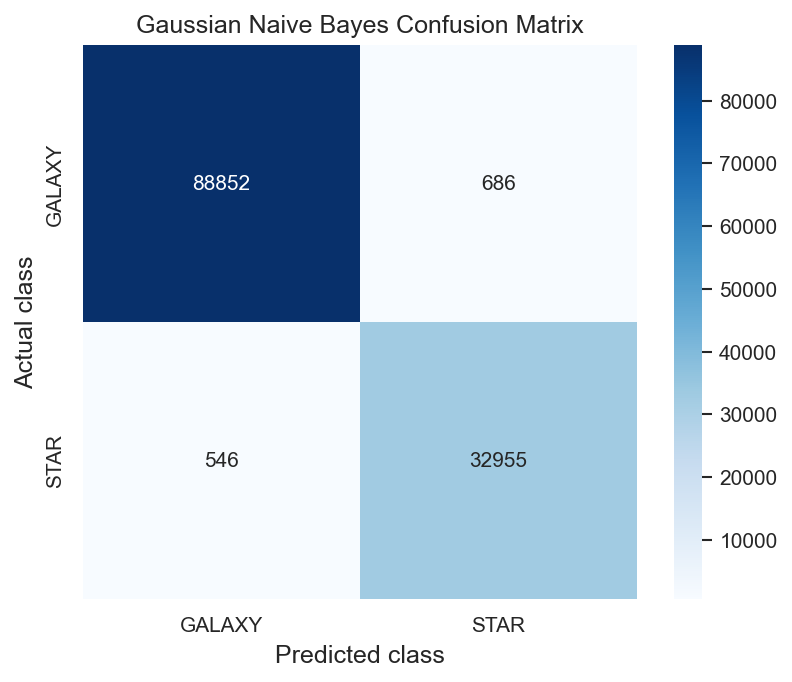
\includegraphics[width=90mm]{gaussian_nb_cm.png}
\caption{Matrica konfuzije za Gaussian Naive Bayes model na test skupu}
\label{fig:gaussian_nb_cm}
\end{figure}

\section{Zaključak}

\begin{figure}[H]
    \centering
    \includegraphics[width=150mm]{conclusion.png}
    \caption{Rezultati korišćenih modela}
    \label{fig:enter-label}
\end{figure}

Na osnovu ovih rezultata, možemo zaključiti da je Random Forest model pokazao najbolje performanse u svim evaluacionim metrikama. Decision Tree se takođe može smatrati dobrom alternativom zbog svojih visokih performansi i jednostavnosti interpretacije.

Ipak, moramo napomenuti da ne postoji univerzalno najbolji model u realnom svetu. Kao što je George E.P. Box jednom rekao: „Svi modeli su pogrešni, ali neki su korisni.“ Važno je samo pronaći model koji je najkorisniji za konkretan problem i podatke.

\newpage
\begin{thebibliography}{Literatura}
\bibitem{} Pang-Ning Tan - Introduction to Data Mining (2019, Pearson Education Limited)
\bibitem{} The SuperCOSMOS Sky Survey - I. Introduction and description (2001) by N. Hambly, H. MacGillivray, M. Read, S. Tritton, E. Thomson, D. Kelly, D. Morgan, R. Smith, S. Driver, J. Williamson, Q. Parker, M. Hawkins, P. Williams and A. Lawrence
\bibitem{} The SuperCOSMOS Sky Survey. Paper II: Image detection, parameterisation, classification and photometry (2001) by N. Hambly, M. Irwin and H. MacGillivray
\bibitem{} Identifying galaxies, quasars, and stars with machine learning: A new catalogue of classifications for 111 million SDSS sources without spectra A. O. Clarke, A. M. M. Scaife, R. Greenhalgh and V. Griguta
\bibitem{} Probst, P.; Wright, M.N.; Boulesteix, A.L. Hyperparameters and tuning strategies for random forest. Wiley Interdiscip. Rev. Data Min. Knowl. Discov. 2019, 9, 1301.
\bibitem{} Xu, B.; Huang, J.Z.; Williams, G.; Wang, Q.; Ye, Y. Classifying very high-dimensional data with random forests built from small subspaces. Int. J. Data Warehous. Min. **2012**, 8, 44–63.
\bibitem{} Javeed, A.; Zhou, S.; Yongjian, L.; Qasim, I.; Noor, A.; Nour, R. An intelligent learning system based on random search algorithm and optimized random forest model for improved heart disease detection.
\end{thebibliography}

\end{document}
